\subsection{\acl{swav}}\label{subsec:SwAV}

\citet{swav_2020} proposed a novel approach to mine positive samples, called \ac{swav}.
It is an online clustering algorithm that works on batches of any size.
If the batch size $B$ is too small to form $K$ clusters the instances are augmented 
with instances from a previous batch, 
but only the original $B$ instances are considered in the loss function.
The approach forces the clusters to have roughly the same size, i.e. form an equipartition.

\citeauthor{swav_2020} claim their method needs neither a memory bank nor a momentum encoder.
The positive sample $x_{nt}$ for an instance $x_n$ is obtained by applying a 
random augmentation $t \in \mathcal{T}$ to $x_n$.
After embedding both the original and the augmented instance, clustering is performed and 
the loss function is computed as defined in \eqref{eq:swav_loss}.
Opposed to other methods, this approach does not directly encourage similar embeddings but similar 
cluster assignments for positive pairs.
However, if both views are similarly encoded they should obtain the same cluster assignment.

\begin{equation}
    L(z_n, z_{nt}) = l(z_n, q_{nt}) + l(z_{nt}, q_n)
    \label{eq:swav_loss}
\end{equation}

The soft cluster assignments $q_n, q_{nt}$ for $x_n, x_{nt}$ respectively 
are used with the other instance's embedding to compute the loss.
The idea is to swap the assignments between the two views of the same image to encourage 
similar cluster assignments for similar instances as illustrated in \autoref{fig:swav_vs_cl}.
The loss $l(z_n, q_{nt})$ is a cross-entropy loss that uses the similarity between the prototype 
of the desired cluster and the embedding of the instance $z_n$ as the probability in the logarithm.

\begin{figure}[h] % h = here, t = top, b = bottom, p = page of floats
    \centering
    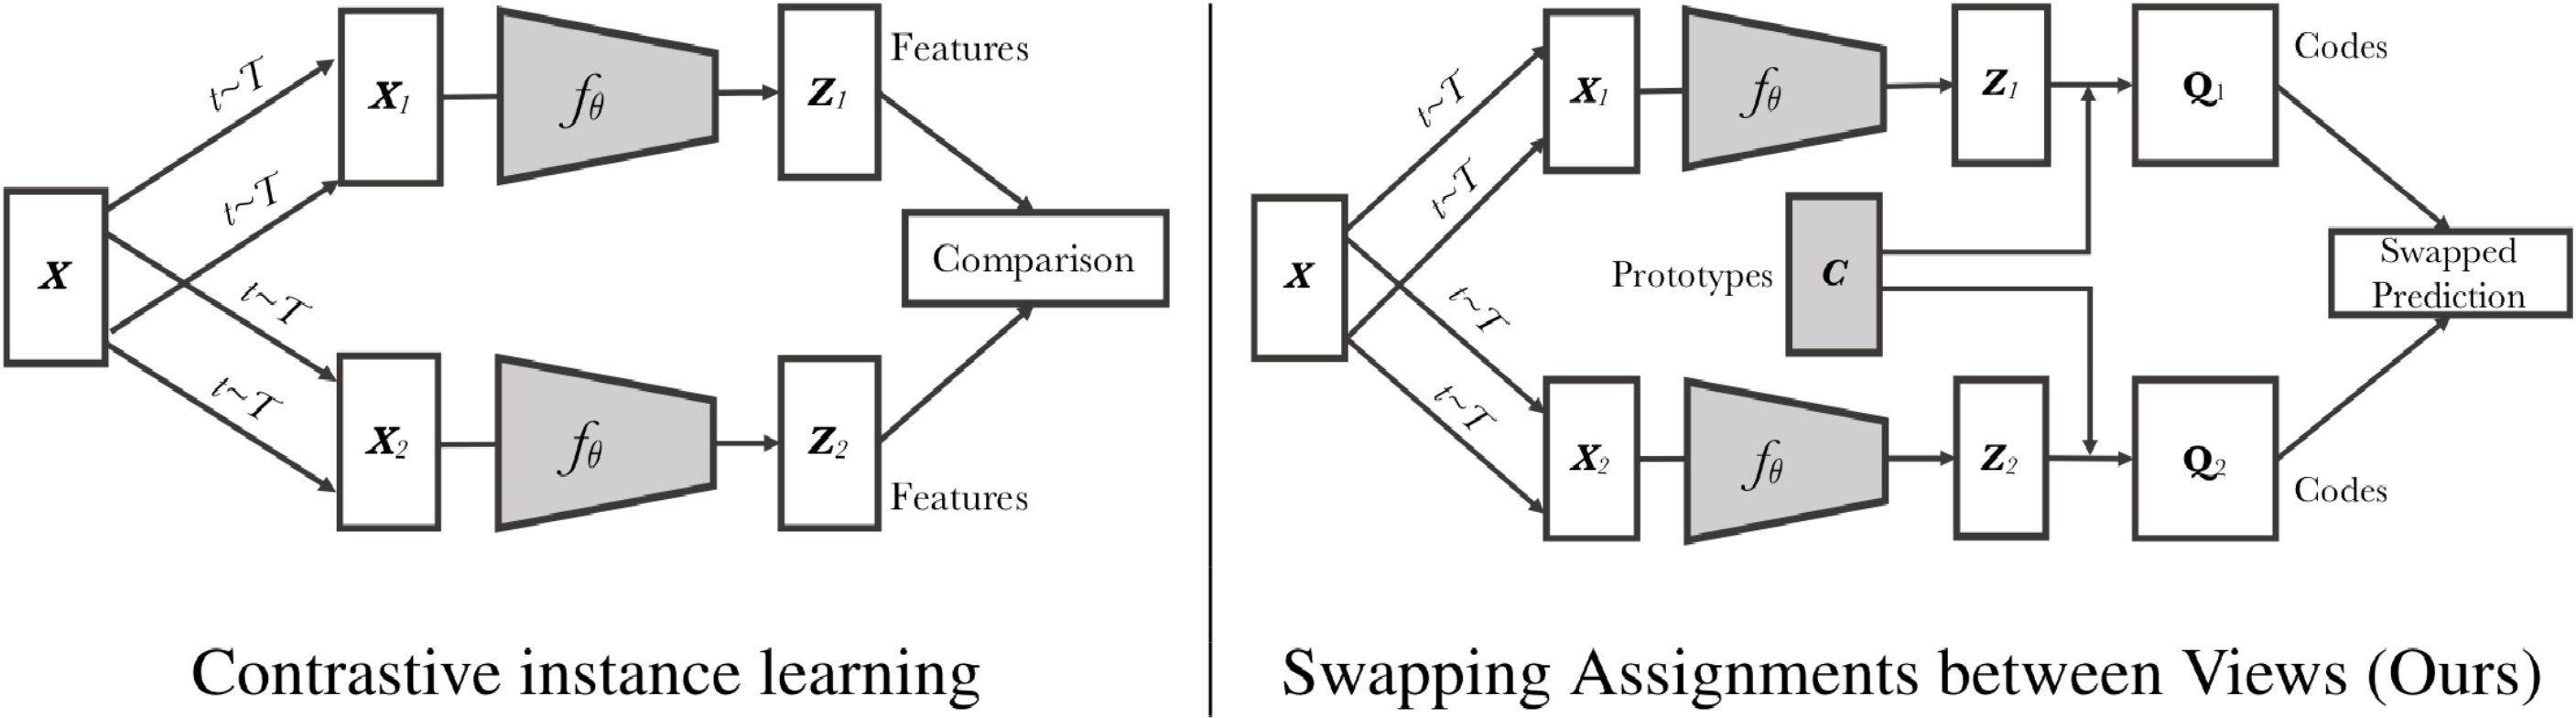
\includegraphics[width=300pt]{images/SwAV_vs_CL.png}
    \caption{Comparison of \ac{cl} and \ac{swav} from \citet{swav_2020}.
    \ac{cl} compares the augmented views directly while 
    \ac{swav} compares cluster assignments.
    Moreover, \ac{swav} computes the loss for an image and the cluster assignments of a positive augmentation 
    rather than its assignments and vice versa.}
    \label{fig:swav_vs_cl}
\end{figure}

\citeauthor{swav_2020} also introduce multi-crop, an augmentation technique that uses different 
crops of the same image.
They include two crops of standard size and standard resolution, 
and $V$ smaller size and low-resolution augmentations.
The resulting loss function is defined in \eqref{eq:swav_loss_multicrop}.

\begin{equation}
    L(z_{t_{1}}, \cdots , z_{t_{V+2}})= \sum_{i\in \left\{ 1,2 \right\} }^{}\sum_{v=1}^{V+2} L_{v \neq i}(z_{t_{v}}, q_{t_{i}})
    \label{eq:swav_loss_multicrop}
\end{equation}